\documentclass{article}
\usepackage[english]{babel}
\usepackage{url}
\usepackage{geometry} %this is for anything that needs geometry like \vspace{x} :) 
\usepackage{natbib}
\usepackage{amsmath}
\usepackage{amsfonts} 
\usepackage{subcaption}
\usepackage{xcolor}
\usepackage{tikz}
\usepackage{caption}
\usepackage{float}
\usepackage{fancyhdr}
\usepackage{setspace}
\bibliographystyle{apalike2}

\tikzset{every picture/.style={line width=0.75pt}} %set default line width to 0.75pt
\geometry{a4paper, left=35mm, right=30mm, top=20mm, bottom=20mm}
\renewcommand{\arraystretch}{1.2}

\doublespacing
\setlength\parindent{24pt}
\allowdisplaybreaks

\begin{document}

\pagestyle{fancy}
\fancyhead[R]{}
\fancyhead[L]{THE MONTY HALL PROBLEM}
\fancyhead[C]{}
\fancyfoot[L]{Mathematics Analysis and Approaches\\ Internal Assessment
for the International Baccalaureate Diploma}
\fancyfoot[R]{candidate number\\ student code}
\renewcommand{\headrulewidth}{0.4pt}
\renewcommand{\footrulewidth}{2pt}

%--------------------------------------
\begin{center}
    \LARGE{\textbf{A graphical description of the Monty Hall problem for an arbitrary number of doors, prizes and opened doors}}
\end{center}
\section*{Introduction}
The aim of this exploration is to get a better understanding of, and solve the famously known Monty Hall problem through an explanation of the problem, getting a better grasp on conditional probability. The concrete aim of this paper is to know if and when it is always beneficial to change doors within the confines of the problem in the context of the original game show. A graphical representation of the problem aims to show the different instances in which the problem is favorable.
\par
This problem disturbed me when starting statistics. This led to an obsessive need to understand the problem logically. Seeing many different depictions of the problem has helped me to logically understand it and therefore conditional probability. After understanding the problem, I wondered how this could be represented outside of the common examples in which it is represented. I specifically wondered if graphing this exact problem could lead to a deeper understanding of it. The nature of the problem is the difficulty in grasping the concept of conditional probability. The Monty Hall problem was my personal approach to improve my understanding of conditional probability, and understanding it has helped me excel in the topic.
\par
The Monty Hall problem serves as a problem within the realm of probability, drawing inspiration from the American television show \textit{Let's Make a Deal}, with its namesake being Monty Hall, the show's original host. This puzzling scenario was made famous through a correspondence written by Steve Selvin and published in the American Statistician in 1975 (\cite{Stev-1975}). The problems revolve around the idea that the guest has to choose between 3 doors. Behind one of the three doors is a prize (originally described as a new car), and behind the two other doors is an undesirable prize (originally represented by goats). After picking one of the 3 doors (and not opening it), the host then opens another door, always showing a goat/undesirable. The question then is should the guest stick to his original door or switch to the other unopened door to have a greater chance of winning the prize.
\par
Many puzzles and brain teases use conditional probability. Many people struggle to grasp this concept, and extending the Monty Hall problem variables not only helps us to understand the solution behind it, but also conditional probability as a whole. A multitude of probabilistic riddles use this exact concept to misdirect. This problem is relevant in many cases, and conditional probability itself is useful even today, being crucial in environments such as medicine and programming, where it is useful to check for diagnostic pathways and error codes within a system respectively(\cite{ackerman2019computability} and \cite{temple2021conditional}).

%--------------------------------------
\section*{Introduction to probability}
Probability is an area of math where the chances of events are studied. Since this paper revolves around probability, clarification of notation is in order, since the ladder may vary depending on regions and areas of math.
\par
A prerequisite is that when talking about probability, the values given of an event happening are restricted between zero and one, with zero meaning that there are no chances of the event happening and one meaning that we can say with certainty that the event will happen. The probability of a given event in a domain $X$ that gives a result $x$ will be annotated as $\mathbb{P}(x)$. Here, the notation $\mathbb{P}(X=x)$ indicates that x is a discrete random variable, which means that X is the sum of the probabilities of all the sample points in a range A that are assigned the value x. Another notation used in this article includes $\neg$, which stands for the opposite or complement of an event $x$, notated as $\neg x$. For example, the probability of a coin landing head is $\mathbb{P}(x)$, while, if described with the same variables, the probability of landing tails would be $\mathbb{P}(\neg x)$ (these understandings are from \cite{jaynes2003probability}).
An important concept in probability that will be used throughout this paper is the difference between mutually exclusive, independent, and dependent events. Mutually exclusive events are events that cannot occur at the same time. For example, the color of a car being red and the color of a car being blue. Independent events are events where the outcome of one event has no effect on the probability of the second even, as, for example, the probability outcome of two separate dice. Dependent events, in contrast, are by definition events that affect each other, exemplified best by examples such as robbing a bank and going to jail. This introduces us to another area of probability, called conditional probability.


%--------------------------------------
\section*{Understanding of conditional probability}
Conditional probability is the probability that an event A occurs, given that it lies within another event B. This means that for two events to have a conditional probability, they must be either independent or dependant (they could be mutually exclusive, but the conditional probability would be 0). The formula for it is as follows:
\begin{equation}
    \mathbb{P}(A \mid B)=\frac{\mathbb{P}(A \cap B)}{\mathbb{P}(B)}
\end{equation}
Conditional probability is notated by a bar place between two given variables as shown in the equation. Conditional probability is all about understanding the probability that an event $A$ is happening, given that an event $B$ is true. It could be logical; now we know that B has occurred and what the new P(A) is. The definition of conditional probability is; the probability of an event occurring given that another event has already occurred. We understand those to be different when probabilities are dependent. We know intuitively that the probability of raining is different from the probability of raining in September. It is important to distinguish how independent and dependent probabilities interplay with conditional probability. As an example, let us take sample group X, where a third of the sample is made up of women, and a third of sample group X also wears glasses. An example of conditional probability in this context would be; What is the probability of a random person from the sample group X wearing glasses, given that they are women. We could assume that the number of women wearing glasses is one third; however, it is not known what percentage of women wear glasses as the distribution of people wearing glasses. Given that the probabilities are independent, we can assume that the probability of women wearing glasses is one-third. In a second instance, where the probability is dependent, we receive additional information that less than a third of the men in the sample group wear glasses. This tells us that the probability that women wear glasses is more than a third. This is the main difference when we talk about conditional probability. It is necessary to know whether the probabilities are independent or dependent. A very intuitive way to look at conditional probability is through a diagram. A diagram can show how each instance acts in the presence of conditional probability.

\begin{figure}[H]
\centering
    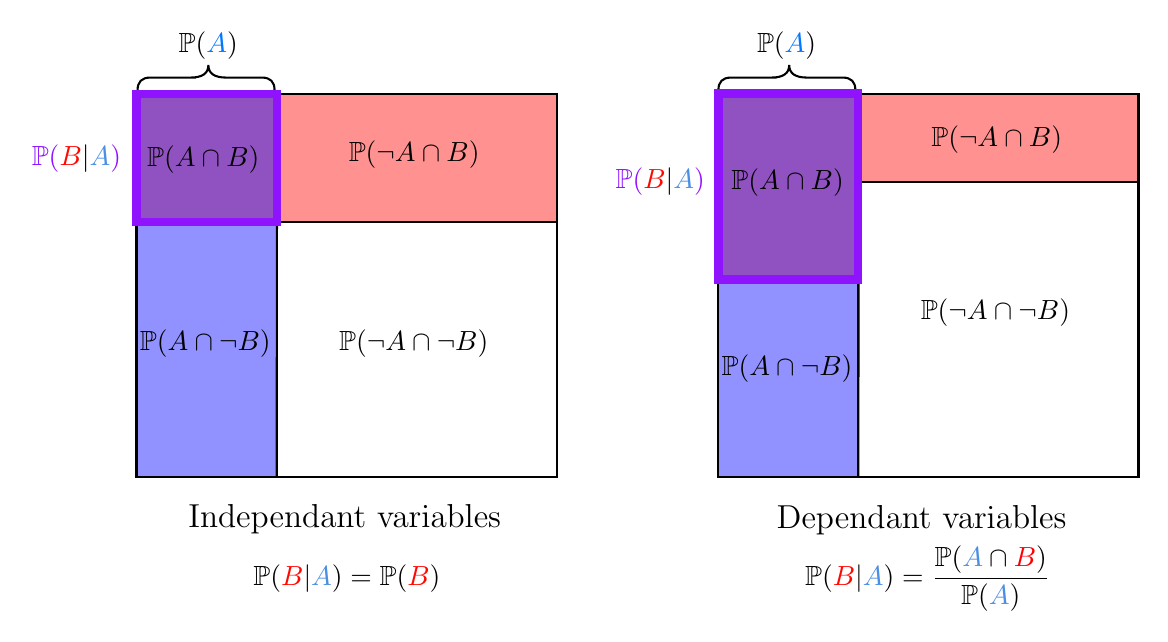
\begin{tikzpicture}[x=0.65pt,y=0.65pt,yscale=-1,xscale=1]
    %uncomment if require: \path (0,382); %set diagram left start at 0, and has height of 382
    
    %Shape: Rectangle [id:dp7813580551740993] 
    \draw   (80.71,47.65) -- (314.36,47.65) -- (314.36,260.7) -- (80.71,260.7) -- cycle ;
    %Straight Lines [id:da860253334870061] 
    \draw    (158.88,47.78) -- (158.59,260.84) ;
    %Straight Lines [id:da5840380251676399] 
    \draw    (80.13,118.8) -- (314.36,118.8) ;
    %Shape: Brace [id:dp2994593708081501] 
    \draw   (157.44,45.67) .. controls (157.44,41) and (155.11,38.67) .. (150.44,38.67) -- (130.65,38.67) .. controls (123.98,38.67) and (120.65,36.34) .. (120.65,31.67) .. controls (120.65,36.34) and (117.32,38.67) .. (110.65,38.67)(113.65,38.67) -- (88.29,38.67) .. controls (83.62,38.67) and (81.29,41) .. (81.29,45.67) ;
    %Shape: Brace [id:dp13942569373516023] 
    \draw   (480.33,45.67) .. controls (480.33,41) and (478,38.67) .. (473.33,38.67) -- (453.54,38.67) .. controls (446.87,38.67) and (443.54,36.34) .. (443.54,31.67) .. controls (443.54,36.34) and (440.21,38.67) .. (433.54,38.67)(436.54,38.67) -- (411.18,38.67) .. controls (406.51,38.67) and (404.18,41) .. (404.18,45.67) ;
    %Shape: Rectangle [id:dp46984634836482375] 
    \draw  [fill={rgb, 255:red, 255; green, 0; blue, 0 }  ,fill opacity=0.43 ] (80.86,47.78) -- (158.88,47.78) -- (158.88,118.93) -- (80.86,118.93) -- cycle ;
    %Shape: Rectangle [id:dp8460341581513102] 
    \draw  [fill={rgb, 255:red, 255; green, 0; blue, 0 }  ,fill opacity=0.43 ] (158.88,47.78) -- (314.36,47.78) -- (314.36,118.8) -- (158.88,118.8) -- cycle ;
    %Shape: Rectangle [id:dp6457590684693343] 
    \draw  [fill={rgb, 255:red, 0; green, 0; blue, 255 }  ,fill opacity=0.43 ] (80.71,47.5) -- (158.59,47.5) -- (158.59,260.84) -- (80.71,260.84) -- cycle ;
    %Shape: Rectangle [id:dp6229852858910147] 
    \draw   (404.09,47.65) -- (637.73,47.65) -- (637.73,260.7) -- (404.09,260.7) -- cycle ;
    %Straight Lines [id:da4279086945487519] 
    \draw    (482.26,47.78) -- (481.97,260.84) ;
    %Straight Lines [id:da16177962386018496] 
    \draw    (482.26,96.5) -- (637.73,96.5) ;
    %Shape: Rectangle [id:dp6829818415900238] 
    \draw  [fill={rgb, 255:red, 255; green, 0; blue, 0 }  ,fill opacity=0.43 ] (404.23,47.78) -- (482.26,47.78) -- (482.26,151) -- (404.23,151) -- cycle ;
    %Shape: Rectangle [id:dp9344115237340047] 
    \draw  [fill={rgb, 255:red, 255; green, 0; blue, 0 }  ,fill opacity=0.43 ] (482.26,47.65) -- (637.73,47.65) -- (637.73,96.5) -- (482.26,96.5) -- cycle ;
    %Shape: Rectangle [id:dp1920401623963076] 
    \draw  [fill={rgb, 255:red, 0; green, 0; blue, 255 }  ,fill opacity=0.43 ] (404.09,47.5) -- (481.97,47.5) -- (481.97,260.84) -- (404.09,260.84) -- cycle ;
    %Shape: Rectangle [id:dp39580990511231673] 
    \draw  [color={rgb, 255:red, 144; green, 19; blue, 254 }  ,draw opacity=1 ][line width=3]  (80.71,47.65) -- (158.88,47.65) -- (158.88,118.93) -- (80.71,118.93) -- cycle ;
    %Shape: Rectangle [id:dp7552921995543582] 
    \draw  [color={rgb, 255:red, 144; green, 19; blue, 254 }  ,draw opacity=1 ][line width=3]  (404.23,47.5) -- (481.97,47.5) -- (481.97,151) -- (404.23,151) -- cycle ;
    
    % Text Node
    \draw (20.77,74.34) node [anchor=north west][inner sep=0.75pt]   [align=left] {$\displaystyle \textcolor[rgb]{0.56,0.07,1}{\mathbb{P}}\textcolor[rgb]{0.56,0.07,1}{(}\textcolor[rgb]{1,0.03,0}{B} |\textcolor[rgb]{0.29,0.56,0.89}{A}\textcolor[rgb]{0.56,0.07,1}{)}$};
    % Text Node
    \draw (107.79,274.07) node [anchor=north west][inner sep=0.75pt]   [align=left] {{\large Independant variables }};
    % Text Node
    \draw (434.87,274.67) node [anchor=north west][inner sep=0.75pt]   [align=left] {{\large Dependant variables }};
    % Text Node
    \draw (80.88,176.86) node [anchor=north west][inner sep=0.75pt]   [align=left] {$\displaystyle \mathbb{P}( A\cap \neg B)$};
    % Text Node
    \draw (191.62,177.12) node [anchor=north west][inner sep=0.75pt]   [align=left] {$\displaystyle \mathbb{P}( \neg A\cap \neg B)$};
    % Text Node
    \draw (258.9,91.59) node [anchor=north west][inner sep=0.75pt]   [align=left] {$ $};
    % Text Node
    \draw (196.98,72.18) node [anchor=north west][inner sep=0.75pt]   [align=left] {$\displaystyle \mathbb{P}( \neg A\cap B)$};
    % Text Node
    \draw (84.85,74.56) node [anchor=north west][inner sep=0.75pt]   [align=left] {$\displaystyle \mathbb{P}( A\cap B)$};
    % Text Node
    \draw (404.25,190.86) node [anchor=north west][inner sep=0.75pt]   [align=left] {$\displaystyle \mathbb{P}( A\cap \neg B)$};
    % Text Node
    \draw (514.99,160.12) node [anchor=north west][inner sep=0.75pt]   [align=left] {$\displaystyle \mathbb{P}( \neg A\cap \neg B)$};
    % Text Node
    \draw (582.28,91.59) node [anchor=north west][inner sep=0.75pt]   [align=left] {$ $};
    % Text Node
    \draw (520.85,63.68) node [anchor=north west][inner sep=0.75pt]   [align=left] {$\displaystyle \mathbb{P}( \neg A\cap B)$};
    % Text Node
    \draw (409.72,87.56) node [anchor=north west][inner sep=0.75pt]   [align=left] {$\displaystyle \mathbb{P}( A\cap B)$};
    % Text Node
    \draw (423.94,11.5) node [anchor=north west][inner sep=0.75pt]   [align=left] {$\displaystyle \mathbb{P}(\textcolor[rgb]{0,0.47,1}{A})$};
    % Text Node
    \draw (102.44,11.5) node [anchor=north west][inner sep=0.75pt]   [align=left] {$\displaystyle \mathbb{P}(\textcolor[rgb]{0,0.47,1}{A})$};
    % Text Node
    \draw (144,308) node [anchor=north west][inner sep=0.75pt]   [align=left] {$\displaystyle \mathbb{P}(\textcolor[rgb]{1,0.03,0}{B} |\textcolor[rgb]{0.29,0.56,0.89}{A}) =\mathbb{P}(\textcolor[rgb]{1,0.03,0}{B})$};
    % Text Node
    \draw (450.67,297.34) node [anchor=north west][inner sep=0.75pt]   [align=left] {$\displaystyle \mathbb{P}(\textcolor[rgb]{1,0.03,0}{B} |\textcolor[rgb]{0.29,0.56,0.89}{A}) =\frac{\mathbb{P}(\textcolor[rgb]{0.29,0.56,0.89}{A} \cap \textcolor[rgb]{1,0,0}{B})}{\mathbb{P}(\textcolor[rgb]{0.29,0.56,0.89}{A})}$};
    % Text Node
    \draw (345.33,87) node [anchor=north west][inner sep=0.75pt]   [align=left] {$\displaystyle \mathbb{\textcolor[rgb]{0.56,0.07,1}{P}}\textcolor[rgb]{0.56,0.07,1}{(}\textcolor[rgb]{1,0.03,0}{B} |\textcolor[rgb]{0.29,0.56,0.89}{A}\textcolor[rgb]{0.56,0.07,1}{)}$};
    \end{tikzpicture}
\caption{Diagram of dependent and independent variables represented in the areas} 
\label{fig: Diagram of dependent and independent variables represented in the areas}
\end{figure}

\par
Now to understand conditional probability, look at the shaded areas of the diagram in figure \ref{fig: Diagram of dependent and independent variables represented in the areas}. The red and blue areas are there to help visualize the different proportions (purple signifies the junction of both blue and red). In the left drawing, it can be seen that the ratio of red (including the area that is purple) in the sample space is equal to the ratio of red area within the blue area (so effectively the ratio of purple area within the blue and purple area since, by definition, all overlap between red and blue is purple). However, if we look at the second diagram, the same areas are not equal, where although the ratios are roughly the same for the sample space, they are not equally distributed with respect to each other compared to the sample space. Using the diagram to aid in the explanation, the conditional probability that the event $B$ occurs since it is $A$ (or $\mathbb{P}(B\mid A)$) would be the ratio between the purple values ($\mathbb{P}(A\cap B)$) divided by the blue area ($\mathbb{P}(A)$ or $\mathbb{P}(A\cap B) + \mathbb{P}(A\cap \neg B)$). What the right diagram describes is the inequality between $\mathbb{P}(A\mid B)$ and $\mathbb{P}(B\mid A)$, and therefore the dependent nature of the variables.

%--------------------------------------
\section*{Models}
\subsection*{The Monty Hall problem}
The famous Monty Hall problem originally has 3 doors. The game host presents you with a choice. One of the doors has a prize behind it (in the original game show, the prize was a car). After choosing one of the doors, the game hosts opens a door, revealing what is behind it (excluding the door you chose). The door cannot be the one you picked, nor the door with the prize. The door opened by the host always has an undesirable (in the original game show, the undesirable was a goat). The game hosts then asks you if you want to keep your original door choice or if you would like to switch doors. 
\par
The first choice for the Monty Hall problem is straight forward, as it is equally probable (probability is distributed equally). The chance of initially choosing the right door is $\frac{1}{3}$. We know that this probability is equally probable throughout all doors. As the host opens a door, and then asks you if you would like to switch, the probabilities change. Deferring from the thought that the probability in this case is 0.5, what must be noticed is the influence of the first choice on the second probability. It may be useful to use a diagram in this case, as we will be referring to the doors multiple times.

\begin{figure}[H]
\centering
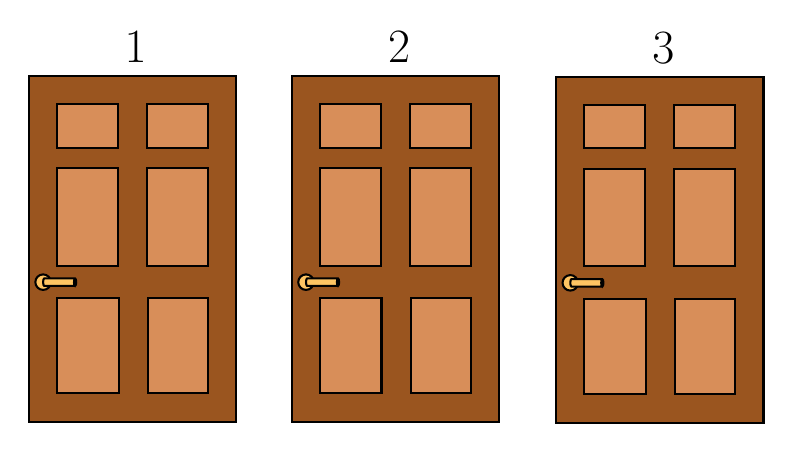
\begin{tikzpicture}[x=0.5pt,y=0.5pt,yscale=-1,xscale=1]
%Shape: Rectangle
\draw  [fill={rgb, 255:red, 154; green, 85; blue, 31 }  ,fill opacity=1 ] (90,50.33) -- (240,50.33) -- (240,300.16) -- (90,300.16) -- cycle ;
%Shape: Rectangle
\draw  [fill={rgb, 255:red, 216; green, 142; blue, 89 }  ,fill opacity=1 ] (110.2,70.53) -- (154.53,70.53) -- (154.53,101.96) -- (110.2,101.96) -- cycle ;
%Shape: Rectangle
\draw  [fill={rgb, 255:red, 216; green, 142; blue, 89 }  ,fill opacity=1 ] (175.6,70.53) -- (219.33,70.53) -- (219.33,101.92) -- (175.6,101.92) -- cycle ;
%Shape: Rectangle
\draw  [fill={rgb, 255:red, 216; green, 142; blue, 89 }  ,fill opacity=1 ] (110.2,116.93) -- (154.53,116.93) -- (154.53,187.16) -- (110.2,187.16) -- cycle ;
%Shape: Rectangle 
\draw  [fill={rgb, 255:red, 216; green, 142; blue, 89 }  ,fill opacity=1 ] (175.6,116.93) -- (219.33,116.93) -- (219.33,187.16) -- (175.6,187.16) -- cycle ;
%Shape: Rectangle 
\draw  [fill={rgb, 255:red, 216; green, 142; blue, 89 }  ,fill opacity=1 ] (110.6,210.76) -- (154.93,210.76) -- (154.93,279.56) -- (110.6,279.56) -- cycle ;
%Shape: Rectangle  
\draw  [fill={rgb, 255:red, 216; green, 142; blue, 89 }  ,fill opacity=1 ] (176,210.76) -- (219.73,210.76) -- (219.73,279.56) -- (176,279.56) -- cycle ;
%Shape: Circle  
\draw  [fill={rgb, 255:red, 255; green, 197; blue, 99 }  ,fill opacity=1 ] (94.8,199.16) .. controls (94.8,196.07) and (97.31,193.56) .. (100.4,193.56) .. controls (103.49,193.56) and (106,196.07) .. (106,199.16) .. controls (106,202.25) and (103.49,204.76) .. (100.4,204.76) .. controls (97.31,204.76) and (94.8,202.25) .. (94.8,199.16) -- cycle ;
%Shape: Can  
\draw  [fill={rgb, 255:red, 255; green, 197; blue, 99 }  ,fill opacity=1 ] (123.53,201.83) -- (101.2,201.83) .. controls (100.76,201.83) and (100.4,200.64) .. (100.4,199.16) .. controls (100.4,197.68) and (100.76,196.49) .. (101.2,196.49) -- (123.53,196.49) .. controls (123.97,196.49) and (124.33,197.68) .. (124.33,199.16) .. controls (124.33,200.64) and (123.97,201.83) .. (123.53,201.83) .. controls (123.09,201.83) and (122.73,200.64) .. (122.73,199.16) .. controls (122.73,197.68) and (123.09,196.49) .. (123.53,196.49) ;
%Shape: Rectangle  
\draw  [fill={rgb, 255:red, 154; green, 85; blue, 31 }  ,fill opacity=1 ] (280,50.33) -- (430,50.33) -- (430,300.16) -- (280,300.16) -- cycle ;
%Shape: Rectangle  
\draw  [fill={rgb, 255:red, 216; green, 142; blue, 89 }  ,fill opacity=1 ] (300.2,70.53) -- (344.53,70.53) -- (344.53,101.96) -- (300.2,101.96) -- cycle ;
%Shape: Rectangle  
\draw  [fill={rgb, 255:red, 216; green, 142; blue, 89 }  ,fill opacity=1 ] (365.6,70.53) -- (409.33,70.53) -- (409.33,101.92) -- (365.6,101.92) -- cycle ;
%Shape: Rectangle  
\draw  [fill={rgb, 255:red, 216; green, 142; blue, 89 }  ,fill opacity=1 ] (300.2,116.93) -- (344.53,116.93) -- (344.53,187.16) -- (300.2,187.16) -- cycle ;
%Shape: Rectangle  
\draw  [fill={rgb, 255:red, 216; green, 142; blue, 89 }  ,fill opacity=1 ] (365.6,116.93) -- (409.33,116.93) -- (409.33,187.16) -- (365.6,187.16) -- cycle ;
%Shape: Rectangle  
\draw  [fill={rgb, 255:red, 216; green, 142; blue, 89 }  ,fill opacity=1 ] (300.6,210.76) -- (344.93,210.76) -- (344.93,279.56) -- (300.6,279.56) -- cycle ;
%Shape: Rectangle  
\draw  [fill={rgb, 255:red, 216; green, 142; blue, 89 }  ,fill opacity=1 ] (366,210.76) -- (409.73,210.76) -- (409.73,279.56) -- (366,279.56) -- cycle ;
%Shape: Circle  
\draw  [fill={rgb, 255:red, 255; green, 197; blue, 99 }  ,fill opacity=1 ] (284.8,199.16) .. controls (284.8,196.07) and (287.31,193.56) .. (290.4,193.56) .. controls (293.49,193.56) and (296,196.07) .. (296,199.16) .. controls (296,202.25) and (293.49,204.76) .. (290.4,204.76) .. controls (287.31,204.76) and (284.8,202.25) .. (284.8,199.16) -- cycle ;
%Shape: Can  
\draw  [fill={rgb, 255:red, 255; green, 197; blue, 99 }  ,fill opacity=1 ] (313.53,201.83) -- (291.2,201.83) .. controls (290.76,201.83) and (290.4,200.64) .. (290.4,199.16) .. controls (290.4,197.68) and (290.76,196.49) .. (291.2,196.49) -- (313.53,196.49) .. controls (313.97,196.49) and (314.33,197.68) .. (314.33,199.16) .. controls (314.33,200.64) and (313.97,201.83) .. (313.53,201.83) .. controls (313.09,201.83) and (312.73,200.64) .. (312.73,199.16) .. controls (312.73,197.68) and (313.09,196.49) .. (313.53,196.49) ;
%Shape: Rectangle  
\draw  [fill={rgb, 255:red, 154; green, 85; blue, 31 }  ,fill opacity=1 ] (471,50.83) -- (621,50.83) -- (621,300.66) -- (471,300.66) -- cycle ;
%Shape: Rectangle  
\draw  [fill={rgb, 255:red, 216; green, 142; blue, 89 }  ,fill opacity=1 ] (491.2,71.03) -- (535.53,71.03) -- (535.53,102.46) -- (491.2,102.46) -- cycle ;
%Shape: Rectangle [id:dp740363394615178] 
\draw  [fill={rgb, 255:red, 216; green, 142; blue, 89 }  ,fill opacity=1 ] (556.6,71.03) -- (600.33,71.03) -- (600.33,102.42) -- (556.6,102.42) -- cycle ;
%Shape: Rectangle [id:dp06578175740868841] 
\draw  [fill={rgb, 255:red, 216; green, 142; blue, 89 }  ,fill opacity=1 ] (491.2,117.43) -- (535.53,117.43) -- (535.53,187.66) -- (491.2,187.66) -- cycle ;
%Shape: Rectangle [id:dp6112889187514874] 
\draw  [fill={rgb, 255:red, 216; green, 142; blue, 89 }  ,fill opacity=1 ] (556.6,117.43) -- (600.33,117.43) -- (600.33,187.66) -- (556.6,187.66) -- cycle ;
%Shape: Rectangle [id:dp9125948028824117] 
\draw  [fill={rgb, 255:red, 216; green, 142; blue, 89 }  ,fill opacity=1 ] (491.6,211.26) -- (535.93,211.26) -- (535.93,280.06) -- (491.6,280.06) -- cycle ;
%Shape: Rectangle [id:dp9713309174471091] 
\draw  [fill={rgb, 255:red, 216; green, 142; blue, 89 }  ,fill opacity=1 ] (557,211.26) -- (600.73,211.26) -- (600.73,280.06) -- (557,280.06) -- cycle ;
%Shape: Circle [id:dp11730381812941759] 
\draw  [fill={rgb, 255:red, 255; green, 197; blue, 99 }  ,fill opacity=1 ] (475.8,199.66) .. controls (475.8,196.57) and (478.31,194.06) .. (481.4,194.06) .. controls (484.49,194.06) and (487,196.57) .. (487,199.66) .. controls (487,202.75) and (484.49,205.26) .. (481.4,205.26) .. controls (478.31,205.26) and (475.8,202.75) .. (475.8,199.66) -- cycle ;
%Shape: Can [id:dp9373972508650583] 
\draw  [fill={rgb, 255:red, 255; green, 197; blue, 99 }  ,fill opacity=1 ] (504.53,202.33) -- (482.2,202.33) .. controls (481.76,202.33) and (481.4,201.14) .. (481.4,199.66) .. controls (481.4,198.18) and (481.76,196.99) .. (482.2,196.99) -- (504.53,196.99) .. controls (504.97,196.99) and (505.33,198.18) .. (505.33,199.66) .. controls (505.33,201.14) and (504.97,202.33) .. (504.53,202.33) .. controls (504.09,202.33) and (503.73,201.14) .. (503.73,199.66) .. controls (503.73,198.18) and (504.09,196.99) .. (504.53,196.99) ;

% Text Node
\draw (157,16) node [anchor=north west][inner sep=0.75pt]   [align=left] {{\LARGE 1}};
% Text Node
\draw (347.5,16) node [anchor=north west][inner sep=0.75pt]   [align=left] {{\LARGE 2}};
% Text Node
\draw (538.5,16.5) node [anchor=north west][inner sep=0.75pt]   [align=left] {{\LARGE 3}};


\end{tikzpicture}
\caption{The Monty Hall problem} 
\label{fig: Diagram of the Monty Hall problem}
\end{figure}

Using the diagram to aid our explanation, let us take the first door chosen to be door 1. The probability that the prize is behind door 1 is $\frac{1}{3}$. Let us say that the hosts opens the door number 2, and that behind it there is an undesirable (as we have already established, the host can only open doors that have the undesirable behind it). The choice we now have is to keep our original choice of door 1, or to switch to door 3. This, as mentioned previously, is not an equally distributed probability. The probability that the prize is behind door 1 remains $\frac{1}{3}$, while the probability that the door is behind door 2 or 3 is capped at door 3, as we now know that door 2 contains an undesirable. This gives us the probability of $\frac{2}{3}$ for door 3, and therefore the best course of action is to switch doors.
\par
One other way to make this switch more obvious is by increasing the number of doors. If we had instead 100 doors and one prize, the switch would be more obvious. If we choose door 1, and the host opens doors 2 through 99, it is clear that it is better to switch to door 100.

\subsection*{Mathematical model of the exploration}
The Monty Hall problem can be logically described with variables. Recall that the probability of an event with a desired discrete outcome x, equally distributed, and a discrete sample space A is;
\begin{equation}
    \mathbb{P}(x)=\frac{n(x)}{n(A)}
\end{equation}
This can be applied to the first choice in the Monty Hall problem, where $n(\textbf{A})$ represents the number of doors or choices, and $n(\textbf{x})$ represents the number of cars/prizes (desirables). For ease of understanding, we will use variables for these. Let $n(\textbf{x})$ be equal to x and $n(\textbf{A})$ be equal to y. The host opens z number of doors (which, as we know, contain undesirables). The probability of us having picked the wrong door in the first place would be the following.
\begin{equation}
    \mathbb{P}(A)=\frac{y-x}{y}
\end{equation}
Now, if we consider the action of switching to a door, the number of doors that we could swap to would be $y-z-1$ remaining doors since we cannot switch to our own door, and also since we cannot switched to an already opened door. The number of doors remaining prized will be $x$ or $x-1$ depending on the first choice. As seen in the equation, the number of doors opened is $z$. This means that the probability that we switch doors and win would be:
\begin{equation}
    \mathbb{P}(A)=\frac{\text{number of remaining prized doors}}{y-z-1}
\end{equation}
This is best shown through a tree diagram, where $\mathbb{P}(C)$ stands for the probability of choosing a prized door to begin with, and $\mathbb{P}(SW)$ stands for the probability of switching door and winning, with its complementary or opposite part being notated as $\mathbb{P}(SL)$ (which is the probability of switching and losing).

\begin{figure}[H]
\centering
    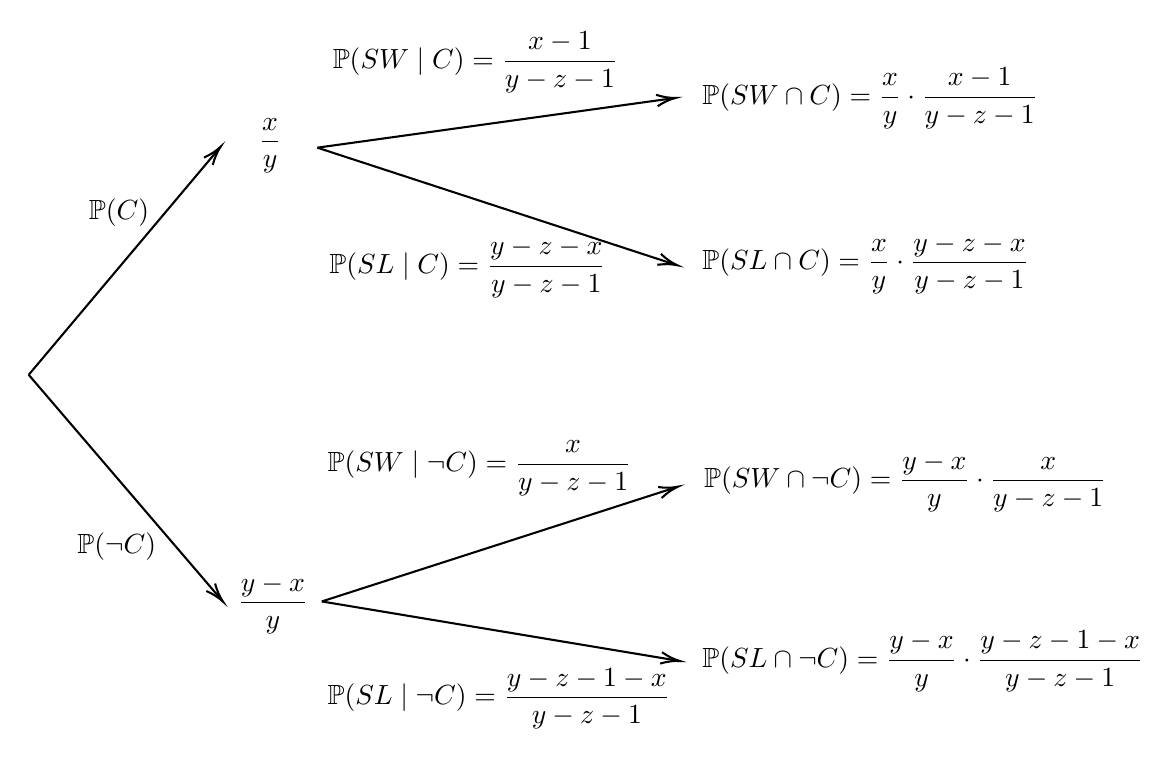
\begin{tikzpicture}[x=0.63pt,y=0.63pt,yscale=-1,xscale=1]
    \draw    (6,221) -- (116.2,349.65) ;
    \draw [shift={(117.5,351.17)}, rotate = 229.42] [color={rgb, 255:red, 0; green, 0; blue, 0 }  ][line width=0.75]    (10.93,-3.29) .. controls (6.95,-1.4) and (3.31,-0.3) .. (0,0) .. controls (3.31,0.3) and (6.95,1.4) .. (10.93,3.29)   ;
    \draw    (6,221) -- (114.81,91.7) ;
    \draw [shift={(116.09,90.17)}, rotate = 130.08] [color={rgb, 255:red, 0; green, 0; blue, 0 }  ][line width=0.75]    (10.93,-3.29) .. controls (6.95,-1.4) and (3.31,-0.3) .. (0,0) .. controls (3.31,0.3) and (6.95,1.4) .. (10.93,3.29)   ;
    \draw    (171.56,90.73) -- (376.04,157.55) ;
    \draw [shift={(377.95,158.17)}, rotate = 198.1] [color={rgb, 255:red, 0; green, 0; blue, 0 }  ][line width=0.75]    (10.93,-3.29) .. controls (6.95,-1.4) and (3.31,-0.3) .. (0,0) .. controls (3.31,0.3) and (6.95,1.4) .. (10.93,3.29)   ;
    \draw    (171.56,90.73) -- (375.14,62.44) ;
    \draw [shift={(377.12,62.17)}, rotate = 172.09] [color={rgb, 255:red, 0; green, 0; blue, 0 }  ][line width=0.75]    (10.93,-3.29) .. controls (6.95,-1.4) and (3.31,-0.3) .. (0,0) .. controls (3.31,0.3) and (6.95,1.4) .. (10.93,3.29)   ;
    \draw    (174.11,351) -- (377.53,384.84) ;
    \draw [shift={(379.5,385.17)}, rotate = 189.44] [color={rgb, 255:red, 0; green, 0; blue, 0 }  ][line width=0.75]    (10.93,-3.29) .. controls (6.95,-1.4) and (3.31,-0.3) .. (0,0) .. controls (3.31,0.3) and (6.95,1.4) .. (10.93,3.29)   ;
    \draw    (174.11,351) -- (376.5,285.78) ;
    \draw [shift={(378.4,285.17)}, rotate = 162.14] [color={rgb, 255:red, 0; green, 0; blue, 0 }  ][line width=0.75] (10.93,-3.29).. controls (6.95,-1.4) and (3.31,-0.3) .. (0,0) .. controls (3.31,0.3) and (6.95,1.4) .. (10.93,3.29)   ;
    \draw (32.18,310) node [anchor=north west][inner sep=0.75pt]   [align=left] {$\displaystyle \mathbb{P}( \neg C)$};
    \draw (136.25,72) node [anchor=north west][inner sep=0.75pt]   [align=left] {$\displaystyle \frac{x}{y}$};
    \draw (123.96,334) node [anchor=north west][inner sep=0.75pt]   [align=left] {$\displaystyle \frac{y-x}{y}$};
    \draw (38.72,118.5) node [anchor=north west][inner sep=0.75pt]   [align=left] {$\displaystyle \mathbb{P}( C)$};
    \draw (178.65,22.5) node [anchor=north west][inner sep=0.75pt]   [align=left] {$\displaystyle \mathbb{P}( SW\mid C) =\frac{x-1}{y-z-1}$};
    \draw (176.65,141) node [anchor=north west][inner sep=0.75pt]   [align=left] {$\displaystyle \mathbb{P}( SL\mid C) =\frac{y-z-x}{y-z-1}$};
    \draw (175.65,257) node [anchor=north west][inner sep=0.75pt]   [align=left] {$\displaystyle \mathbb{P}( SW\mid\neg C) =\frac{x}{y-z-1}$};
    \draw (175.65,387.5) node [anchor=north west][inner sep=0.75pt]   [align=left] {$\displaystyle \mathbb{P}( SL\mid\neg C) =\frac{y-z-1-x}{y-z-1}$};
    \draw (390.65,43) node [anchor=north west][inner sep=0.75pt]   [align=left] {$\displaystyle \mathbb{P}( SW\cap C) =\frac{x}{y} \cdot \frac{x-1}{y-z-1}$};
    \draw (390.65,139) node [anchor=north west][inner sep=0.75pt]   [align=left] {$\displaystyle \mathbb{P}( SL\cap C) =\frac{x}{y} \cdot \frac{y-z-x}{y-z-1}$};
    \draw (391.65,264) node [anchor=north west][inner sep=0.75pt]   [align=left] {$\displaystyle \mathbb{P}( SW\cap \neg C) =\frac{y-x}{y} \cdot \frac{x}{y-z-1}$};
    \draw (390.65,366) node [anchor=north west][inner sep=0.75pt]   [align=left] {$\displaystyle \mathbb{P}( SL\cap \neg C) =\frac{y-x}{y} \cdot \frac{y-z-1-x}{y-z-1}$};
    \end{tikzpicture}
\caption{Tree diagram of the Monty Hall problem} \label{fig: Tree diagram}
\end{figure}

The tree diagram shows the probabilities involved with the Monty Hall problem. The conditional probabilities here can be found through logical thinking. Although this process is harder when trying to find the probabilities of switching doors and getting an undesirable result, these can still be easily explained. For the probability of $\mathbb{P}(SW\mid C)$, follows the equation $\frac{\text{number of remaining prized doors}}{y-z-1}$, with the available doors being $x-1$. Although the amount of prizes do not change, the first choice being correct eliminates one of the available doors to switch to. Since we cannot switch to the door we have previously chosen, 1 has to be subtracted from the total amount of prizes (prized doors/desired doors). The same logic applies to $\mathbb{P}(SW\mid\neg C)$, but due to the fact that we exclude no prizes (or prized doors/desired doors), the total number of doors containing prizes/desirables continues to be $x$. For $\mathbb{P}(SL\mid C)$ and $\mathbb{P}(SL\mid\neg C)$, we subtract the available doors ($y-z-1$) by the number of remaining prized doors. Since we have already found the number of remaining prized doors, the subsequent probabilities are straightforward.
\par
Importantly, the interjection of probabilities can be found through the equation for conditional probability. It is important to note that this only works since the probability of switching and winning is fully within the probability of having chosen a prized door in the first place. The equation used for the determination of the interjection is the aforementioned one:
\begin{equation}
\begin{aligned}
\mathbb{P}(A \mid B)=\frac{\mathbb{P}(A \cap B)}{\mathbb{P}(B)}
\end{aligned}
\end{equation}
This equation gives use a mean of calculating the interjection with our available probabilities. Using the same notation as the diagram, the relation between the interjection and the other probabilities can be seen.
\begin{equation}
\begin{aligned}
\mathbb{P}(C)\cdot\mathbb{P}(SW\mid C)=\mathbb{P}(SW \cap C)
\end{aligned}
\end{equation}
The same relation can be used to found all four interjections we have. Through the interjection, we can calculate the probability of winning (having a prized door) while having switched. Since the probability of $SW$ is composed with respect to $C$ and $\neg C$, we can assume $\mathbb{P}(SW)=\mathbb{P}(SW\mid C)+\mathbb{P}(SW\mid\neg C)$. The calculation for $\mathbb{P}(SW)$ follows:
\begin{equation}
\begin{aligned}
\mathbb{P}(SW)&=\mathbb{P}(SW\mid C)+\mathbb{P}(SW\mid\neg C)\\
\mathbb{P}(SW)&=\frac{x}{y} \cdot \frac{x-1}{y-z-1}+\frac{y-x}{y} \cdot \frac{x}{y-z-1}\\
\mathbb{P}(SW)&=\frac{x}{y} \cdot \frac{x-1}{y-z-1}+\frac{x}{y} \cdot \frac{y-x}{y-z-1}\\
\mathbb{P}(SW)&=\frac{x}{y} \cdot \left(\frac{x-1}{y-z-1}+\frac{y-x}{y-z-1}\right)\\
\mathbb{P}(SW)&=\frac{x}{y} \cdot \left(\frac{y-1}{y-z-1}\right)\\
\mathbb{P}(SW)&=\frac{xy-x}{y(y-z-1)}\\
\end{aligned}
\end{equation}
\par
Parallelly, since we have to assume the problem to be real and cannot subtract more doors than there are, or open more doors than available, the range of the problem is defined through these equations:
\begin{equation}
\begin{aligned}
y \geq x&+1+z\\
x&>1
\end{aligned}
\end{equation}
\par
This concludes the mathematical description of the Monty Hall problem.

%--------------------------------------
\subsection*{Visual model of the exploration through different variables}
Due to the complicated nature of representing a four-dimensional graph on a paper, one of the variables (in this case, z, which represents the amount of doors opened by the host) becomes the parameter $k$. As such, we are able to graph the equation on a three-dimensional graph and use its third axis to output the probability while using the number of opened doors as an interchangeable constant. If we then make the graphs opaque and view them with the z axis pointed towards the outside of the paper, we can see at which values of $x$ and $y$ the probability of switching and winning ($\frac{y x-x}{y(y-k-1)}$) is higher than the probability of winning without switching ($\frac{x}{y}$). It is important to note that we are only interested in the whole number combinations, as our variables are within the $\mathbb{N}$ range. This can be seen in the graph as intersections on the grid. The functions used for the graphs are as follows:

\begin{equation*}
\begin{aligned}
    f_1(x,y) =& \frac{y x-x}{y(y-k-1)} = z\\
    f_2(x,y) =& \frac{x}{y} = z
\end{aligned}
\end{equation*}

The above functions represent $\mathbb{P}(SW)$ and $\mathbb{P}(C)$, $\mathbb{P}(SW)$ being $f_1$, and $\mathbb{P}(C)$ being $f_2$. These have been derived from the previous explanation of the problem, under the "mathematical model of the explanation" section.
\par
In order to distinguish the function, they are colored. The function $f_1$ is colored opaque blue, and $f_2$ is colored purple/violet. What follows is the two functions graphed with k being equal to zero, and the aforementioned figure being figure~\ref{fig:Graphing the Monty Hall problem k0}. Although $k=0$ is not within the range of the Monty Hall problem, this is more an illustrative step.

\begin{figure}[H]
\centering
\includegraphics[width=0.6\textwidth]{img/Presentation2.png}
\caption{Graphing the Monty Hall problem with k=0}
\label{fig:Graphing the Monty Hall problem k0}
\end{figure}

This first graph (Figure~\ref{fig:Graphing the Monty Hall problem k0}) is with the parameter set to 0. Although not yet clear, the two functions are the same in this case. To prove that these are equal, we can equate them by replacing $k$ with zero.
\begin{equation*}
\begin{aligned}
    \frac{x}{y} =& \frac{y x-x}{y(y-1)} \\
    \frac{x\cdot(y(y-1))}{y} =& y x-x \\
    x(y-1) =& y x-x \\
    xy-x =& y x-x \\
    1=1
\end{aligned}
\end{equation*}

However, the following figure is of the same two equations, with $k$ set to one. More importantly, another thing that can be observed in this graph is a red line. The line follows the domain of the problem, with it being $y \geq x+1+k$. The red line follows the equation $y = x+1+k$ considering this to be a two-dimensional graph. This means that everything above it on the $y$ axis is within the range, while everything below is impossible given the domain.

\begin{figure}[H]
\centering
\includegraphics[width=0.6\textwidth]{img/Presentation1.png}
\caption{Graphing the Monty Hall problem with k=1}
\label{fig:Graphing the Monty Hall problem k1}
\end{figure}

In order to clarify, the function that appears from this point of view is further up on the z-axis, which means that it has a higher probability. The color that shows at any point is, therefore, the situation in which the probability of the indicated function is higher for the given number of doors and prizes. In figure~\ref{fig:Graphing the Monty Hall problem k1}, we can see how an increase in $k$ increases the probability ($z$ value) of the function independent of the the $x$ and $y$ values of the functions. We can also see this mathematically, since $k$ reduces the value of the denominator independent of the values of $x$ and $y$ (since $k$ and $y$ are within the range of $\mathbb{N}$). However, it also creates a division between $f_1$ and $f_2$. Although the previous statement still holds (that the probability of $f_1$, or switching and winning increases with $k$), the $z$ axis being a probability has a range between zero and one, creating a division. 
\par
As to prove this division to be insignificant independent of the value of the parameter $k$, we need to prove that this two-dimensional line always is smaller than the range of the problem (in the $y$ axis). We have previously proved that the range of the Monty Hall problem is within $y \geq x+1+k$, $1\geq z\geq0$ and $x>1$, so if we prove that the separating line is smaller than the range of the problem, we can definitively prove that it is always superior to switch doors within the Monty Hall problem. This is only true since, as we have seen, the function $f_1$ as a whole is greater than $f_2$ while $k>1$, apart from the section where $f_1$ is above 1.
\par
Firstly we create the separator line by equating $f_1=1$ and isolating y (with help from \cite{Mathematica}). This is because to equate the range of the problem, we need to create the two-dimensional equation that represents the separating line with the included parameter.

\begin{equation*}
\begin{aligned}
    \frac{1}{2}\left(\sqrt{k^2+2 k x+2 k+x^2-2 x+1}+k+x+1\right) = y
\end{aligned}
\end{equation*}

Now we can equate the separation line with the bounds of the problem. The proof can be shown through simple arithmetic.
\begin{equation*}
\begin{aligned}
    \frac{1}{2}\left(\sqrt{k^2+2 k x+2 k+x^2-2 x+1}+x+1+k\right) &\leq x+1+k\\
    \sqrt{k^2+2 k x+2 k+x^2-2 x+1}+x+1+k &\leq 2(x+1+k)\\
    \sqrt{k^2+2 k x+2 k+x^2-2 x+1} &\leq x+1+k\\
    k^2+2 k x+2 k+x^2-2 x+1 &\leq (x+1+k)^2\\
    k^2+2 k x+2 k+x^2-2 x+1 &\leq k^2 + 2 k x + 2 k + x^2 + 2 x + 1\\
    -2 x &\leq 2 x\\
    -1 &\leq 1\\
\end{aligned}
\end{equation*}

This proof is the culmination of the math that has been done so far. It is concrete evidence that, independent of the number of doors, prizes, and doors opened, it is better, or at the least not detrimental, to switch door in every single case (within the bounds that the problem imposes).

%--------------------------------------
\section*{Conclusion}
The Monty Hall problem has intrigued and puzzled people for years. This exploration sought to shed light on this classic probability puzzle by examining it from mathematical and visual perspectives.
\par
Through the graphical model, we prove that the switch of doors is indeed advantageous. Conditional probability and the manipulation of variables demonstrated that the probability of winning a car increases significantly when choosing to switch.
\par
The visual models provided intuitive insight into the problem. It clearly showed how Monty Hall's actions in opening doors and revealing undesirable outcomes affect the odds of winning the car. These visual models can be powerful tools for both teaching and understanding the Monty-Hall problem.
\par
In conclusion, the Monty Hall problem serves as an excellent example of conditional probability. A challenge to our intuitions and underscore the importance of considering all available information when making choices. The mathematical and visual models presented in this exploration offer different angles for grasping this intriguing problem, making it accessible and engaging for learners of probability and statistics.
\pagebreak
%--------------------------------------
\bibliography{references}

\end{document}